\documentclass{article}

%%% Fill details here (in the second brackets)
\newcommand{\name}{Weijie Gan}     % Your name (First Last)
\newcommand{\wustlkey}{gan.weijie}             % Your WUSTL Key
%%%

%%%%%%%%%%%%%%%%%%%%%% Formatting Stuff %%%%%%%%%%%%%%%%%%%%%%%%%%%
\usepackage{times}
\usepackage[T1]{fontenc}

\setlength{\parskip}{1em}\setlength{\parindent}{0pt}
\linespread{1.25}
\usepackage[margin=0.7in,top=1in]{geometry}\usepackage{fancyhdr}
\pagestyle{fancy}\lhead{\bf \name}\rhead{\bf \wustlkey}\cfoot{\thepage}
\newcommand{\info}{\clearpage \subsection*{Information}}
\newcommand{\solution}[1]{\clearpage \subsection*{Solution #1}}
\newcommand{\spart}[1]{\paragraph{(#1)}}
%%%%%%%%%%%%%%%%%%%%%%%%%%%%%%%%%%%%%%%%%%%%%%%%%%%%%%%%%%%%%%%%%%%

%%% Add any more packages if you want to
\usepackage{amsmath,graphicx}

\begin{document}
%%%%% Main Body goes here
%%%%%-----------------------------------
%%%%%
%%%%%        Solution 1
%%%%%
%%%%%-----------------------------------
% Begin solution to every problem like this.
\solution{1} 
\spart{a} 
From slide, we know that:
$$
I = gI^0 + g \sqrt{I^0} \varepsilon_1 + \sqrt{\bigg (g^2 \sigma_{2a}^2 + \sigma_{2b}^2 \bigg )} \varepsilon_2
$$             
Where both $\varepsilon_1$ and $\varepsilon_2$ is zero-mean Gaussian noise $\mathcal{N}(0,1)$. Thus,
$$
\begin{aligned}
  I & = gI^0 + \mathcal{N}(0,\ g^2 I^0) + \mathcal{N}(0, (g^2 \sigma_{2a}^2 + \sigma_{2b}^2 )) \\
    & = gI^0 + \mathcal{N}(0,\ g^2 I^0 + (g^2 \sigma_{2a}^2 + \sigma_{2b}^2 )) \\
\end{aligned}
$$           
Variance of $\varepsilon_{(a)}$ is $g^2 I^0 + (g^2 \sigma_{2a}^2 + \sigma_{2b}^2)$

\spart{b}
Since $g_{(b)} = g \times k$ and $I_{(b)}^0 = \frac{I^0}{k}$,
$$
\begin{aligned}
  \varepsilon_{(b)} & = \mathcal{N} \bigg (0, \ g_{(b)}^2 I_{(b)}^0 + (g_{(b)}^2 \sigma_{2a}^2 + \sigma_{2b}^2) \bigg )\\
  & = \mathcal{N} \bigg (0, \ {(g \times k)}^2 \frac{I^0}{k} + ({(g \times k)}^2 \sigma_{2a}^2 + \sigma_{2b}^2) \bigg ) \\
  & = \mathcal{N} \bigg (0, \ g^2 k I_0 + g^2 k^2 \sigma_{2a}^2 + \sigma_{2b}^2 \bigg ) \\
\end{aligned}
$$ 
Variance of $\varepsilon_{(b)}$ is $g^2 k I_0 + g^2 k^2 \sigma_{2a}^2 + \sigma_{2b}^2$

\spart{c}
Similar with above excise $(b)$:
$$
\begin{aligned}
  I_k & = gI^0 + \mathcal{N}\bigg ( 0, \  g^2 k I_0 + g^2 k^2 \sigma_{2a}^2 + \sigma_{2b}^2 \bigg) \\
\end{aligned}
$$ 
Since $I = (I_1 + I_2 + ... I_k)/k $:
$$
\begin{aligned}
  I_1 + I_2 + ... I_k & =  k*gI^0 + \sum_k\ \mathcal{N}\bigg ( 0, \  g^2 k I_0 + g^2 k^2 \sigma_{2a}^2 + \sigma_{2b}^2 \bigg) \\
  I & = \frac{1}{k} \bigg( k*gI^0 + \sum_k\ \mathcal{N}\bigg ( 0, \  g^2 k I_0 + g^2 k^2 \sigma_{2a}^2 + \sigma_{2b}^2 \bigg) \bigg) \\
  I & = \frac{1}{k} \bigg( k*gI^0 + \mathcal{N}\bigg ( 0, \  g^2 k^2 I_0 + g^2 k^3 \sigma_{2a}^2 + k \sigma_{2b}^2 \bigg) \\
  I & = gI^0 + \mathcal{N}\bigg ( 0, \ \frac{1}{k^2} (g^2 k^2 I_0 + g^2 k^3 \sigma_{2a}^2 + k \sigma_{2b}^2) \bigg) \\ 
  I & = gI^0 + \mathcal{N}\bigg ( 0, \ g^2 I_0 + g^2 k \sigma_{2a}^2 + \frac{1}{k} \sigma_{2b}^2 \bigg) \\
\end{aligned}
$$ 
Variance of $\varepsilon_{(c)}$ is $g^2 I_0 + g^2 k \sigma_{2a}^2 + \frac{1}{k} \sigma_{2b}^2$

\spart{d}
Because $\varepsilon_{(c)}$ is smaller than $\varepsilon_{(b)}$, I prefer $k$ shots with exposure time $T/k$.
%%%%%-----------------------------------
%%%%%
%%%%%        Solution 2
%%%%%
%%%%%-----------------------------------
\solution{2} 
The answer is shown as figure [\ref{fig:s2-ori}] and figure [\ref{fig:s2-ans}].
\begin{figure*}[!h]
  \centering
  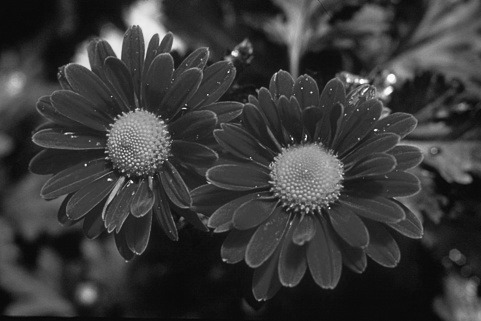
\includegraphics[height=15em]{"code/inputs/p2_inp.jpg"}
  \caption{Solution 2 - Original Image}
  \label{fig:s2-ori}
\end{figure*}
\begin{figure*}[!h]
  \centering
  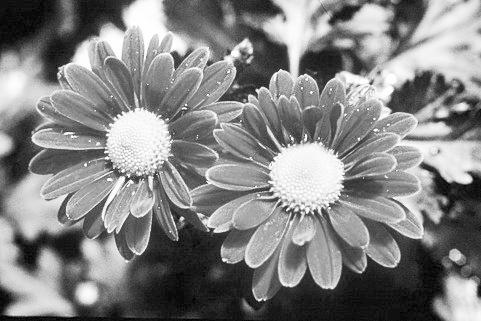
\includegraphics[height=15em]{"code/outputs/prob2.jpg"}
  \caption{Solution 2 - Histogram Equalized Image}
  \label{fig:s2-ans}
\end{figure*}
%%%%%-----------------------------------
%%%%%
%%%%%        Solution 3
%%%%%
%%%%%-----------------------------------
\solution{3}
\spart{a}
The answer is shown as figure [\ref{fig:s3a-ori}] and figure [\ref{fig:s3a-ans}].
\begin{figure*}[!h]
  \centering
  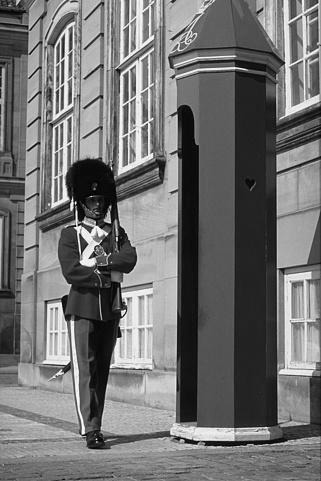
\includegraphics[height=15em]{"code/inputs/p3_inp.jpg"}
  \caption{Solution 3 - Original Image}
  \label{fig:s3a-ori}
\end{figure*}
\begin{figure*}[!h]
  \centering
  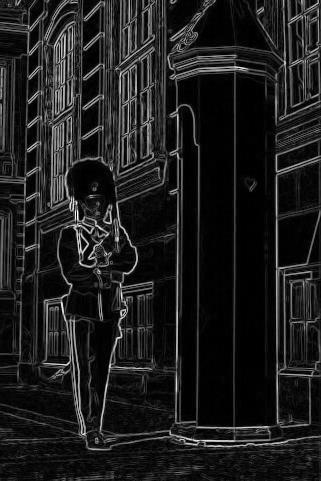
\includegraphics[height=15em]{"code/outputs/prob3_a.jpg"}
  \caption{Solution 3 - Magnitudes $H$ Image}
  \label{fig:s3a-ans}
\end{figure*}
\spart{b}
When threshold value is $T_0 = 0.5$, image before NMS is shown as figure [\ref{fig:s3b0-ori}] and image after NMS is shown as figure [\ref{fig:s3b0-ans}].
When threshold value is $T_1 = 1.0$, image before NMS is shown as figure [\ref{fig:s3b1-ori}] and image after NMS is shown as figure [\ref{fig:s3b1-ans}].
When threshold value is $T_2 = 1.5$, image before NMS is shown as figure [\ref{fig:s3b2-ori}] and image after NMS is shown as figure [\ref{fig:s3b2-ans}].
\begin{figure*}[!h]
  \centering
  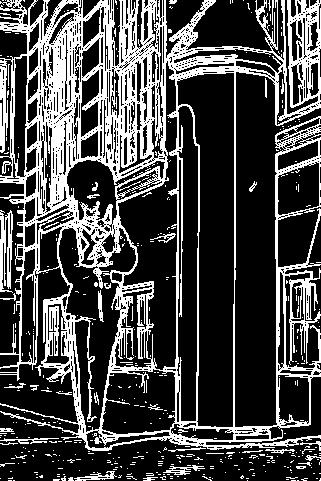
\includegraphics[height=15em]{"code/outputs/prob3_b_0.jpg"}
  \caption{Solution 3 - $T_0 = 0.5$ Before NMS}
  \label{fig:s3b0-ori}
\end{figure*}
\begin{figure*}[!h]
  \centering
  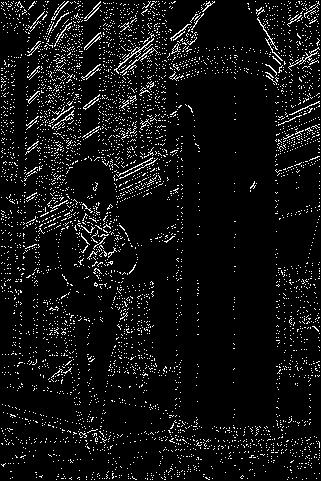
\includegraphics[height=15em]{"code/outputs/prob3_b_nms0.jpg"}
  \caption{Solution 3 - $T_1 = 0.5$ After NMS}
  \label{fig:s3b0-ans}
\end{figure*}
\begin{figure*}[!h]
  \centering
  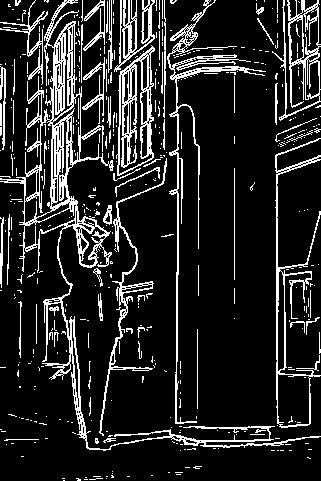
\includegraphics[height=15em]{"code/outputs/prob3_b_1.jpg"}
  \caption{Solution 3 - $T_1 = 1.0$ Before NMS}
  \label{fig:s3b1-ori}
\end{figure*}
\begin{figure*}[!h]
  \centering
  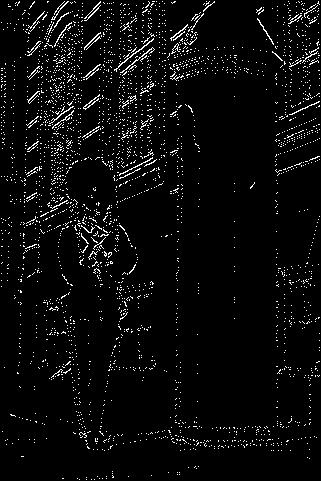
\includegraphics[height=15em]{"code/outputs/prob3_b_nms1.jpg"}
  \caption{Solution 3 - $T_0 = 1.0$ After NMS}
  \label{fig:s3b1-ans}
\end{figure*}
\begin{figure*}[!h]
  \centering
  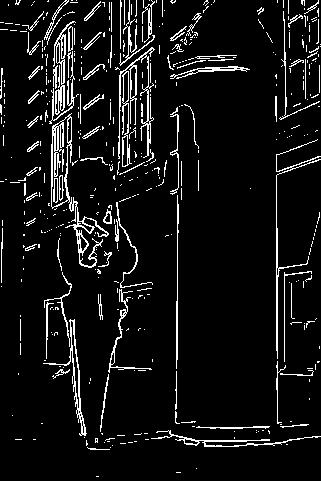
\includegraphics[height=15em]{"code/outputs/prob3_b_2.jpg"}
  \caption{Solution 3 - $T_2 = 1.5$ Before NMS}
  \label{fig:s3b2-ori}
\end{figure*}
\begin{figure*}[!h]
  \centering
  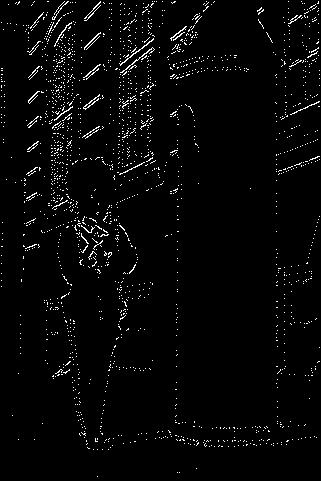
\includegraphics[height=15em]{"code/outputs/prob3_b_nms2.jpg"}
  \caption{Solution 3 - $T_2 = 1.5$ After NMS}
  \label{fig:s3b2-ans}
\end{figure*}
%%%%%-----------------------------------
%%%%%
%%%%%        Solution 4
%%%%%
%%%%%-----------------------------------
\solution{4}
Results are listed as follows.
\begin{figure*}[!h]
  \centering
  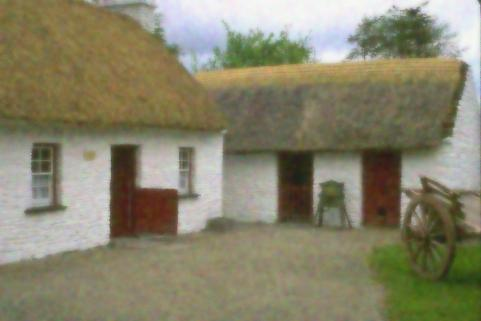
\includegraphics[height=15em]{"code/outputs/prob4_1_a.jpg"}
  \caption{Solution 4 - prob4\_1\_a}
\end{figure*}
\begin{figure*}[!h]
  \centering
  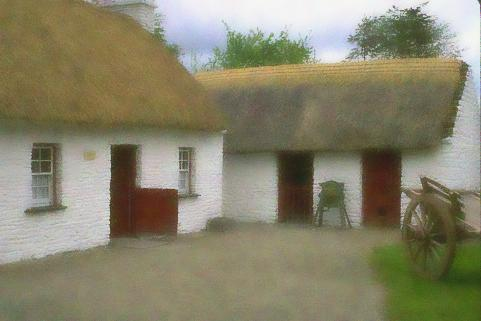
\includegraphics[height=15em]{"code/outputs/prob4_1_b.jpg"}
  \caption{Solution 4 - prob4\_1\_b}
\end{figure*}
\begin{figure*}[!h]
  \centering
  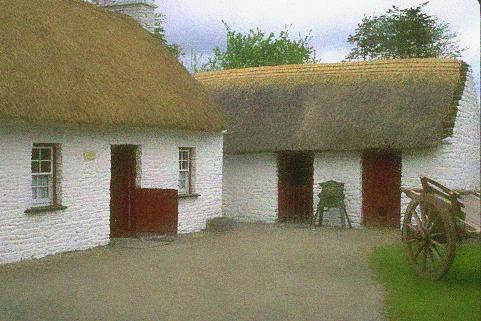
\includegraphics[height=15em]{"code/outputs/prob4_1_c.jpg"}
  \caption{Solution 4 - prob4\_1\_c}
\end{figure*}
\begin{figure*}[!h]
  \centering
  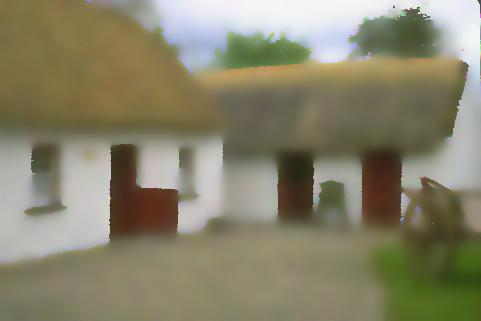
\includegraphics[height=15em]{"code/outputs/prob4_1_rep.jpg"}
  \caption{Solution 4 - prob4\_1\_rep}
\end{figure*}
\begin{figure*}[!h]
  \centering
  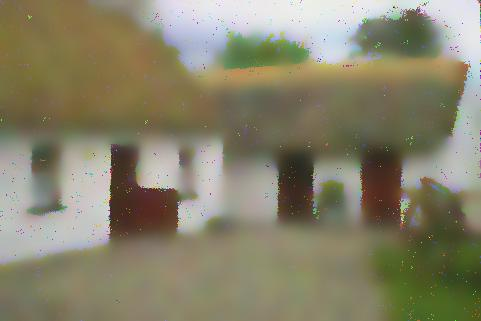
\includegraphics[height=15em]{"code/outputs/prob4_2_rep.jpg"}
  \caption{Solution 4 - prob4\_2\_rep}
\end{figure*}
%%%%%-----------------------------------
%%%%%
%%%%%        Solution 5
%%%%%
%%%%%-----------------------------------
\solution{5} 
\spart{a}
The key idea to solve this problem is: $F[u,v] = \overline{F}[W-u, H-v]$.
Then, when only consider imaginary part, $I(F[u,v]) = -I(F[W-u, H-v])$. When only consider real part, $R(F[u,v]) = R(F[W-u, H-v])$.
Since both real part and imaginary part in $F[u,v]$ are \textbf{central symmetric}, we both can use half of $W\times H$ space to store real part or imaginary part.
All in all, we can ues $W\times H$ space to store $F[u,v]$.

The situation that both width and height are odd is shown as figure [\ref{fig:5a-all-odd}]. 
In a $W\times H$ space, there is a central point $(x_c, y_c)$, $x_c = int(width/2)$ and $y_c = int(height/2)$, which shown as red area in the figure.
The blue area means real part of $F$ and the imaginary part of $F$ is shown as green area.
Also, I think the central point can not be stored with one real scalar.
\begin{figure*}[!h]
  \centering
  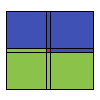
\includegraphics[height=15em]{"./All-odd.png"}
  \caption{Solution 5 - a- All Odd}
  \label{fig:5a-all-odd}
\end{figure*}

The situation that both width and height are even is shown as figure [\ref{fig:5a-all-even}].
Because both are even, a $W\times H$ space can be divided into two equal part, both in vertical and horizontal direction.
The blue area means real part of $F$ and the imaginary part of $F$ is shown as green area. 
\begin{figure*}[!h]
  \centering
  
\includegraphics[height=15em]{"./All-even.png"}
  \caption{Solution 5 - a - All Even}
  \label{fig:5a-all-even}
\end{figure*}

The situation that width or height is odd and the other is even, is shown as figure [\ref{fig:5a-either}]. 
Because width and height is even, a $W\times H$ space can be divided into two equal part, in vertical direction, if height is odd, and horizontal otherwise.
The blue area means real part of $F$ and the imaginary part of $F$ is shown as green area.
\begin{figure*}[!h]
  \centering
  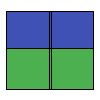
\includegraphics[height=15em]{"./Either.png"}
  \caption{Solution 5 - a - One is Odd and the other is Even}
  \label{fig:5a-either}
\end{figure*}

\spart{b}
Result is shown as follow.
\begin{figure*}[!h]
  \centering
  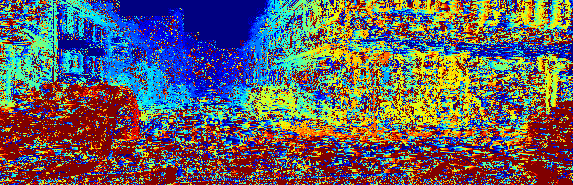
\includegraphics[height=15em]{"code/outputs/prob5.jpg"}
  \caption{Solution 5 - b}
\end{figure*}
%%%%%-----------------------------------
%%%%%
%%%%%        Solution 6
%%%%%
%%%%%-----------------------------------
\solution{6}
\spart{a}
Results are listed as follows.
\begin{figure*}[!h]
  \centering
  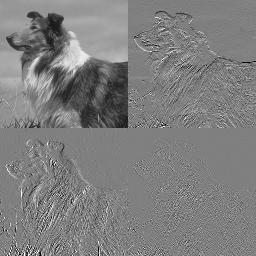
\includegraphics[height=15em]{"code/outputs/prob6a_1.jpg"}
  \caption{Solution 6 - prob6a\_1}
\end{figure*}
\begin{figure*}[!h]
  \centering
  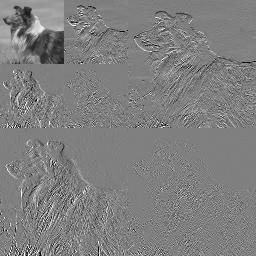
\includegraphics[height=15em]{"code/outputs/prob6a_2.jpg"}
  \caption{Solution 6 - prob6a\_2}
\end{figure*}
\begin{figure*}[!h]
  \centering
  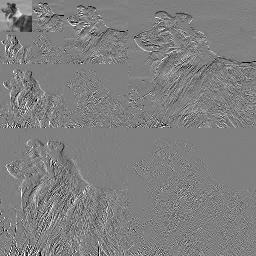
\includegraphics[height=15em]{"code/outputs/prob6a_3.jpg"}
  \caption{Solution 6 - prob6a\_3}
\end{figure*}
\spart{b}
Results are listed as follows.
\begin{figure*}[!h]
  \centering
  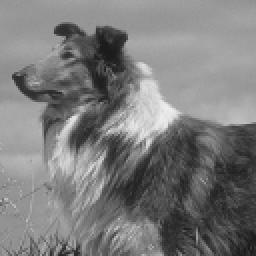
\includegraphics[height=15em]{"code/outputs/prob6b_0.jpg"}
  \caption{Solution 6 - prob6b\_0}
\end{figure*}
\begin{figure*}[!h]
  \centering
  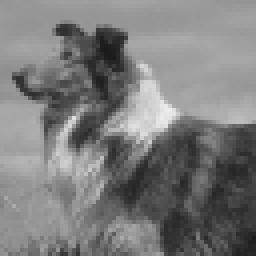
\includegraphics[height=15em]{"code/outputs/prob6b_1.jpg"}
  \caption{Solution 6 - prob6b\_1}
\end{figure*}
\begin{figure*}[!h]
  \centering
  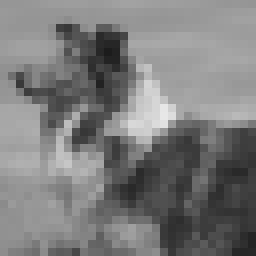
\includegraphics[height=15em]{"code/outputs/prob6b_2.jpg"}
  \caption{Solution 6 - prob6a\_2}
\end{figure*}
%%%%%%%%%% Important, you must edit and complete the informational
%%%%%%%%%% section below. If you discussed the problem set with no
%%%%%%%%%% one, edit it to say no discussions or external resources.
\info

This problem set took approximately 20 hours of effort. And I finish it by myself.

\end{document}
